\documentclass[serif]{beamer}
\usepackage{amsmath,amssymb,amsfonts}
\usepackage{tikz}
\usetheme[block=fill,progressbar=foot,background=light]{metropolis}
\usefonttheme[onlymath]{serif}
\usetikzlibrary{calc,positioning}

%Information to be included in the title page:
\title{BIM2005 Fall 2021}
\subtitle{Principal Component Analysis (PCA): Principle and Implementation}
\author{Haoran Sun (USTF)}
\institute{CUHK-Shenzhen}
\date{November 24, 2021}

\AtBeginSection[]
{
  \begin{frame}<beamer>
    \frametitle{Outline}
    \tableofcontents[currentsection]
  \end{frame}
}

\begin{document}

\frame{\titlepage}

\begin{frame}{Outline}
    \tableofcontents
\end{frame}



\section{Motivation}
\begin{frame}
    \frametitle{Why we reduce the dimension of a dataset?}
    \begin{itemize}
        \item Curse of dimensionality
        \begin{itemize}
            \item Difficult to \alert{understand}: which dimension should we focus on? Where is the slow motion? How is the potential energy?
            \item \alert{Noise} exists: how to eliminate the meaningless fluctuation within a dataset?
            \item Hard to \alert{visualize}: how to understand them intuitively?
        \end{itemize}

        \begin{center}
            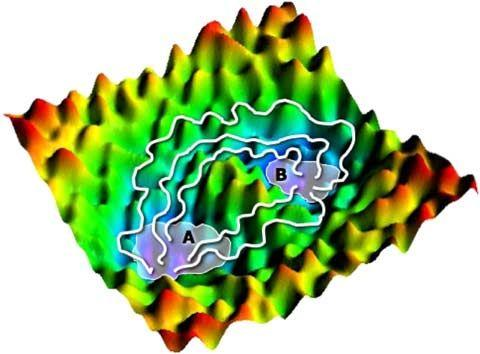
\includegraphics[width=2in]{potential.jpg}
        \end{center}
        % \item Dimensionality reduction
        % \begin{itemize}
        %     \item Find a \alert{discriptive} low dimensional space.
        %     \item Used for visualizing high-dimensional dataset, reduce the $N$-D data to 2-D or 3-D.
        %     \item Identify low-dimensional space that contains \alert{information} as much as possible (or, eliminate the noise).
        % \end{itemize}
    \end{itemize}
\end{frame}

\begin{frame}
    \frametitle{Why we reduce the dimension of a dataset?}
    \begin{itemize}
        % \item Curse of dimensionality
        % \begin{itemize}
        %     \item Difficult to \alert{understand}: which dimension should we focus on? Where is the slow motion?
        %     \item \alert{Noise} exists: how to eliminate the meaningless fluctuation within a dataset?
        %     \item Hard to \alert{visualize}: how to understand them intuitively?
        % \end{itemize}
        \item Dimensionality reduction
        \begin{itemize}
            \item Find a \alert{discriptive} low dimensional space.
            \item Used for visualizing high-dimensional dataset, reduce the $N$-D data to 2-D or 3-D.
            \item Identify low-dimensional space that contains \alert{information} as much as possible (or, eliminate the noise).
        \end{itemize}
        
        \begin{center}
            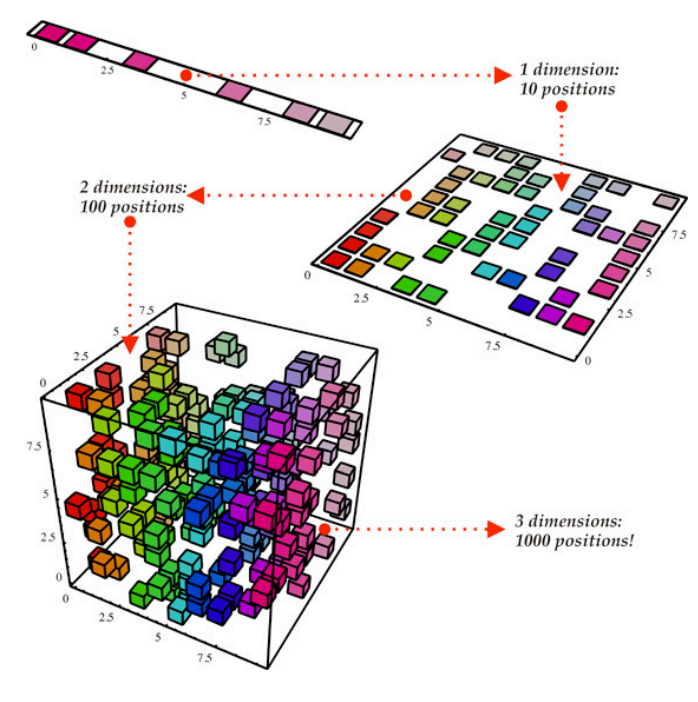
\includegraphics[width=1.5in]{dimreduct.png}
        \end{center}
    \end{itemize}
\end{frame}

\begin{frame}
    \frametitle{Motivation: reduce the dimension by projection}
    \begin{itemize}
        \item Assume that we are going to reduce a 2-D dataset to 1-D by \alert{projection} (MAT2040).
        \begin{center}
            \includegraphics<1>[width=3in]{./proj0.pdf}
            \includegraphics<2>[width=3.5in]{./proj12.pdf}
        \end{center}
        % \item<2> Regarding our question, which of these two is better? Why?
        % \item<1> How to choose the `best' \alert{direction} we project the dataset?
    \end{itemize}
\end{frame}

\begin{frame}
    \frametitle{Motivation: reduce the dimension by projection}
    \begin{itemize}
        \item We want this low-dimensional representation contains information as much as possible.
        % \item It seems that reduced dataset on the left figure spanned more widely. While the data points at the right figure almost packed together.
        \item Which of these reduced datasets contains `more' information?
        \begin{center}
            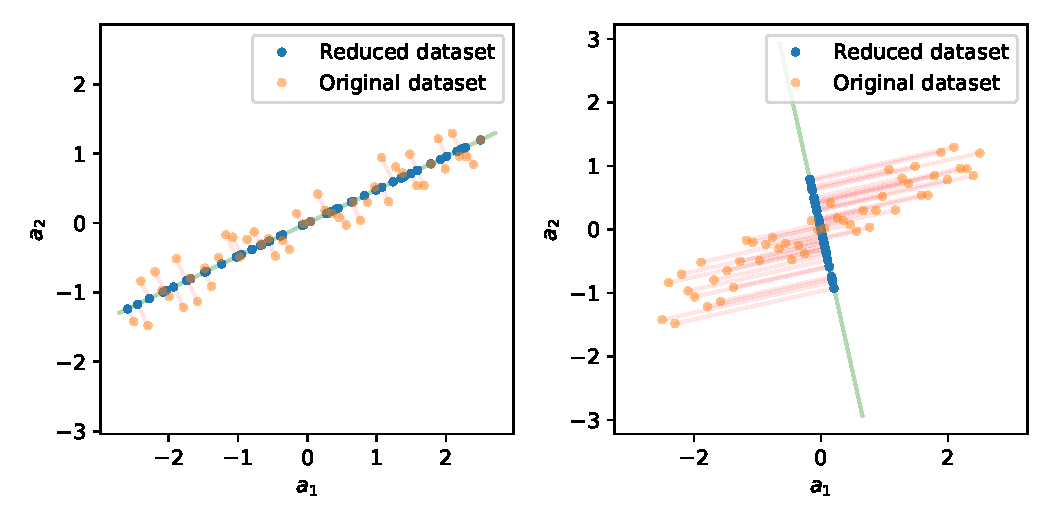
\includegraphics[width=3.5in]{./proj12.pdf}
        \end{center}
    \end{itemize}
\end{frame}

\begin{frame}
    \frametitle{Motivation: choose the standard}
    \begin{itemize}
        \item Intuitively, spanned widely $\rightarrow$ more information.
        \item How to verify `spanned widely' \alert{quantitatively}? By which standard?
        \begin{center}
            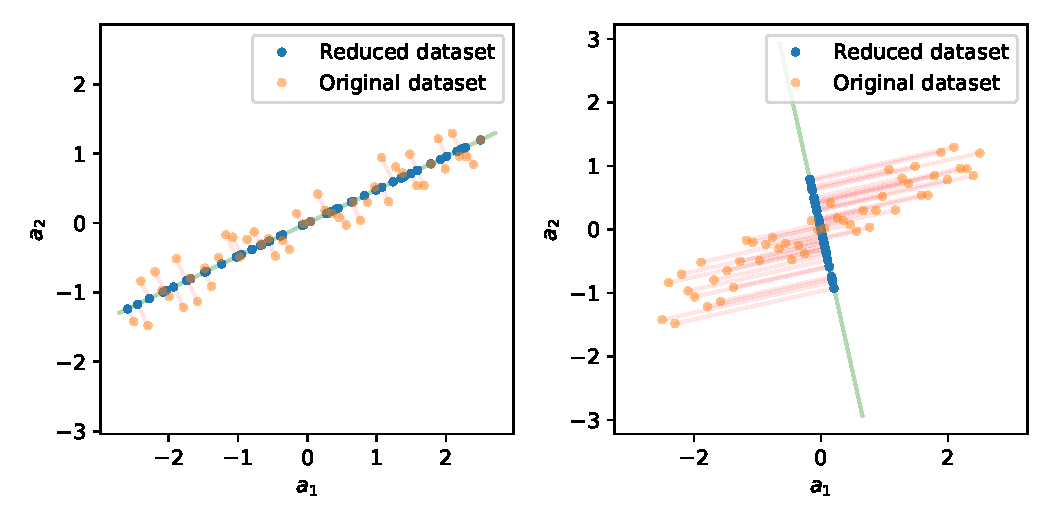
\includegraphics[width=3.5in]{./proj12.pdf}
        \end{center}
    \end{itemize}
\end{frame}

\begin{frame}
    \frametitle{Motivation: choose the standard}
    \begin{itemize}
        \item In statistical inference, \alert{variance} always used as an measurement that how data points spread around their mean value (STA2001).
        \item Thus, reduced dataset on left has higher variance, while the right has lower variance.
        \begin{center}
            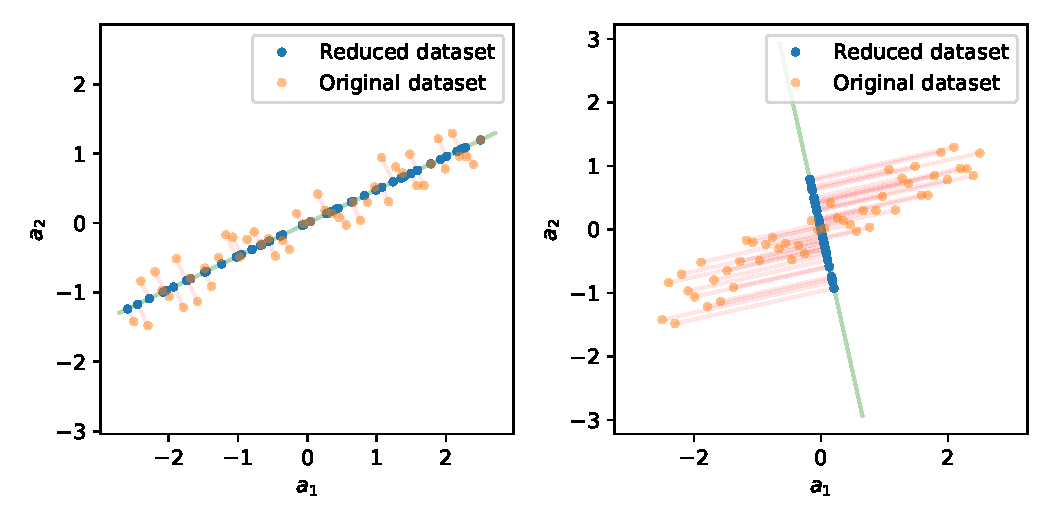
\includegraphics[width=3.5in]{./proj12.pdf}
        \end{center}
    \end{itemize}
\end{frame}

\begin{frame}
    \frametitle{Motivation: choose the standard}
    \begin{itemize}
        \item Therefore, we choose \alert{variance} as the standard when choosing the direction which we are going to project data on.
        \item We want more information $\rightarrow$ we want to get reduced dataset large variance $\rightarrow$ \textbf{we want to maximize variance.}
        \begin{center}
            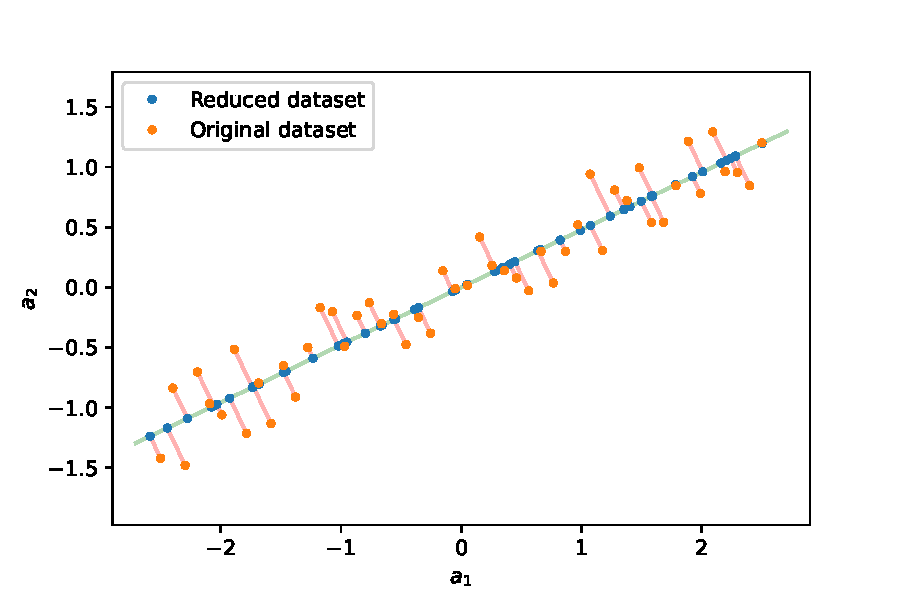
\includegraphics[width=3in]{./proj1.pdf}
        \end{center}
    \end{itemize}
\end{frame}


% \begin{frame}
%     \frametitle{How to choose the most appropriate solution?}
%     Assume that we would like to reduce a 2-D dataset to 1D, how to reduce
% \end{frame}

\section{Mathematical background}
\begin{frame}
    \frametitle{Notations: dataset}
    \begin{itemize}
        \item We have a $d$-D dataset $\mathcal{A}$ contains $N$ data points, represent this dataset as \alert{matrix} $A$.
        \item Each column of a matrix represents a data point (vector).
        $$
        A = \begin{bmatrix}
            \mathbf{a}^{(1)} & \mathbf{a}^{(2)} & \cdots & \mathbf{a}^{(N)}
        \end{bmatrix}\in\mathbb{R}^{d\times N}
        % = \begin{bmatrix}
        %     a_1^{(1)} & a_1^{(2)} & \cdots & a_1^{(N)}\\
        %     a_2^{(1)} & a_2^{(2)} & \cdots & a_2^{(N)}
        % \end{bmatrix}
        $$
        \item $\mathbf{a}^{(i)}$ is the $i$th data point, it could be represented in column vector form.
        $$
        \mathbf{a}^{(i)} = \begin{bmatrix}
            a_1^{(i)}\\ a_2^{(i)}\\ \vdots \\ a_d^{(i)}
        \end{bmatrix}\in\mathbb{R}^{d\times 1}
        $$
    \end{itemize}
\end{frame}

\begin{frame}
    \frametitle{Notations: projection vector}
    \begin{itemize}
        \item We would like to project dataset $\mathcal{A}$ onto a unit vector $\mathbf{x}$, i.e., we project each $\mathbf{a}^{(i)}$ onto $\mathbf{x}$.
        \begin{center}
            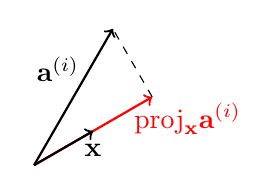
\begin{tikzpicture}
                \coordinate (O) at (0,0);
                \coordinate (A) at (1.50,0.866);
                \coordinate (B) at (1.00,1.732);
                \coordinate (C) at (0.75,0.433);
                \draw[->, thick] (O) -- (B) node[pos=0.7, left ] {$\mathbf{a}^{(i)}$};
                \draw[->, thick, red] (O) -- (A) node[pos=1.3, below=6pt] {$\mathrm{proj}_{\mathbf{x}}\mathbf{a}^{(i)}$};
                \draw[->, thick]   (O) -- (C) node[below=1pt] {$\mathbf{x}$};
                \draw[dashed]    (A) -- (B);
            \end{tikzpicture}
        \end{center}
        \item Since $\mathbf{x}$ is an unit vector, i.e., $\|\mathbf{x}\|=1$, then
        $$
        \mathrm{proj}_{\mathbf{x}}\mathbf{a}^{(i)} = (\mathbf{x}\cdot\mathbf{a}^{(i)})\mathbf{x}
        $$
        where the inner product $\mathbf{x}\cdot\mathbf{a}^{(i)}$ is equivalent to
        $$
        \mathbf{x}\cdot\mathbf{a}^{(i)} = \mathbf{x}^T\mathbf{a}^{(i)}
        $$
        Also
        $$
        \|\mathrm{proj}_{\mathbf{x}}\mathbf{a}^{(i)}\| = \mathbf{x}\cdot\mathbf{a}^{(i)} = \mathbf{x}^T\mathbf{a}^{(i)}
        $$
    \end{itemize}
\end{frame}

\begin{frame}
    \frametitle{Notations: reduced dataset}
    \begin{itemize}
        \item We can build an axis along the unit vector $\mathbf{x}$, using the length of projected vector as coordinate value.
        \begin{center}
            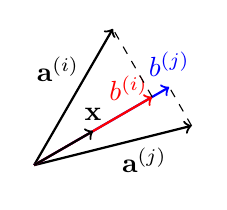
\begin{tikzpicture}
                \coordinate (O) at (0,0);
                \coordinate (A) at (1.50,0.866);
                \coordinate (B) at (1.00,1.732);
                \coordinate (C) at (0.75,0.433);
                \coordinate (D) at (2.00,0.500);
                \coordinate (F) at (1.716,0.991);
                \draw[->, thick] (O) -- (B) node[pos=0.7, left ] {$\mathbf{a}^{(i)}$};
                \draw[->, thick] (O) -- (D) node[pos=0.7, below ] {$\mathbf{a}^{(j)}$};
                \draw[->, thick, blue] (O) -- (F) node[above] {$b^{(j)}$};
                \draw[->, thick, red] (O) -- (A) node[pos=0.8,above] {$b^{(i)}$};
                \draw[->, thick]   (O) -- (C) node[above] {$\mathbf{x}$};
                \draw[dashed]    (A) -- (B);
                \draw[dashed]    (D) -- (F);
            \end{tikzpicture}
        \end{center}
        \item Define \alert{reduced dataset} $\mathcal{B}$ with respect to coordinate $b$, using matrix $B$ to represent $\mathcal{B}$.
        $$
        B = \begin{bmatrix}
            b_1 & b_2 &\cdots & b_N
        \end{bmatrix} = \mathbf{x}^T A = 
        \begin{bmatrix}
            \mathbf{x}^T\mathbf{a}^{(1)} & \cdots & \mathbf{x}^T\mathbf{a}^{(N)}
        \end{bmatrix}
        $$
    \end{itemize}
\end{frame}

\begin{frame}
    \frametitle{Notations: reduced dataset}
    \begin{itemize}
        \item By projection, we can obtain 1-D dataset $\mathcal{B}$ from 2-D dataset $\mathcal{A}$.
        \begin{center}
            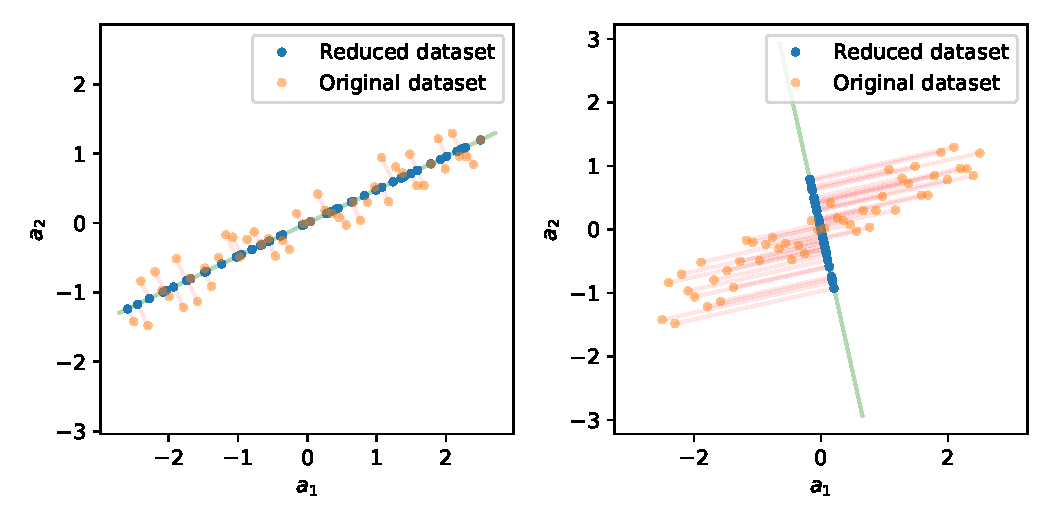
\includegraphics[width=3.5in]{./proj12.pdf}
        \end{center}
    \end{itemize}
\end{frame}

\begin{frame}
    \frametitle{Notations: mean and variance}
    \begin{itemize}
        \item Recall the definition of mean and variance, given a random variable $X$, the mean $\mu$ and variance $\sigma^2$ is defined as
        $$
        \begin{aligned}
            \mu      &= E(X)\\
            \sigma^2 &= E\left[(X - \mu)^2\right]
        \end{aligned}
        $$
    \end{itemize}
\end{frame}

\begin{frame}
    \frametitle{Notations: sample variance}
    \begin{itemize}
        % \item In other words, `$\mathcal{B}$ spanned widely' means `$\mathcal{B}$ exhibits a high variance'.
        \item Recall our goal: \textbf{choosing appropriate unit vector $\mathbf{x}$ which maximize the variance of 1-D dataset $\mathcal{B}$}.
        \item Note that we would use sample variance $S^2_\mathcal{B}$, which is an approximate of variance $\sigma_\mathcal{B}^2$ (we assumed that $\mu_\mathcal{A} = \mathbf{0}$).
        $$
        \begin{aligned}
            \sigma_\mathcal{B}^2 \approx S^2_\mathcal{B} &= \frac{1}{N-1}\sum_{i=1}^N (b^{(i)} - \bar{b})^2 & \\
            &= \frac{1}{N-1}\sum_{i=1}^N {b^{(i)}}^2 & \text{($\bar{b}=0$ if $\mu_\mathcal{A} = \mathbf{0}$)} \\
            &= \frac{1}{N-1}\mathbf{x}^TAA^T\mathbf{x} \approx \frac{1}{N}\mathbf{x}^TAA^T\mathbf{x} & \text{(large $N$)}
        \end{aligned}
        $$
        \item $\mathbf{S} = \displaystyle \frac{1}{N} AA^T$ is usually called the \alert{covariance matrix}.
    \end{itemize}
\end{frame}

\begin{frame}
    \frametitle{Notations: Lagrange multipliers}
    \begin{itemize}
        \item Thus, our question becomes
        \begin{center}
            \centering
            \begin{tabular}{lr}
                Maximize & $S^2_\mathcal{B} = \frac{1}{N}\mathbf{x}^TAA^T\mathbf{x}$\\
                Constrained by & $\|\mathbf{x}\| = 1 \Leftrightarrow \|\mathbf{x}\| - 1 = 0$
            \end{tabular}
        \end{center}
        \item Recall the knowledge in calculus. Generally, we solve extreme problem with constraint by the method of \alert{Lagrange multipliers}.
        \item More specifically, we are going to solve
        \begin{center}
            \centering
            \begin{tabular}{lr}
                Minimize/maximize & $f(\mathbf{x})$\\
                Constrained by & $g(\mathbf{x}) = 0$
            \end{tabular}
        \end{center}
        \item We can solve this problem by define the Lagrange function $\mathcal{L}$, and solve the equation set $\nabla_{\mathbf{x},\lambda}\mathcal{L}=\mathbf{0}$.
        $$
        \mathcal{L}(\mathbf{x}, \lambda) = f(\mathbf{x}) - \lambda g(\mathbf{x}), \nabla_{\mathbf{x},\lambda}\mathcal{L}=\mathbf{0}
        $$
    \end{itemize}
\end{frame}

\begin{frame}
    \frametitle{Simplification}
    \begin{itemize}
        \item To simplify calculation, we modify our problem to
        \begin{center}
            \centering
            \begin{tabular}{lr}
                Maximize & $f(\mathbf{x}) = \mathbf{x}^TAA^T\mathbf{x}$\\
                Constrained by & $g(\mathbf{x}) = \mathbf{x}^T\mathbf{x} - 1 = 0$
            \end{tabular}
        \end{center}
        since $N$ is a constant, $\mathbf{x}^T\mathbf{x} = 1$ is equivalent to $\|\mathbf{x}\|=1$
        \item Therefore, the Lagrange function would be
        $$
        \mathcal{L}(\mathbf{x}, \lambda) = \mathbf{x}^TAA^T\mathbf{x} - \lambda(\mathbf{x}^T\mathbf{x} - 1)
        $$
    \end{itemize}
\end{frame}

\begin{frame}
    \frametitle{Calculate the gradient}
    \begin{itemize}
        \item Note that the gradient would be
        $$
        \nabla_{\mathbf{x},\lambda}\mathcal{L} = 
        \begin{bmatrix}
            \left[\frac{\partial \mathcal{L}}{\partial \mathbf{x}}\right]^T\\
            1 - \mathbf{x}^T\mathbf{x}
        \end{bmatrix} = \mathbf{0}
        $$
        \item It could be shown that
        $$
        \begin{aligned}
            \frac{\partial\mathcal{L}}{\partial \mathbf{x}} &= \frac{\partial [\mathbf{x}^TAA^T\mathbf{x} - \lambda(\mathbf{x}^T\mathbf{x} - 1)]}{\partial \mathbf{x}}\\
            &= 2\mathbf{x}^TAA^T - 2\lambda\mathbf{x}^T = 0\\
            \Rightarrow &AA^T\mathbf{x} = \lambda\mathbf{x}
        \end{aligned}
        $$
        \item Therefore
        $$
        \begin{cases}
            AA^T\mathbf{x} = \lambda\mathbf{x}\\
            1 - \mathbf{x}^T\mathbf{x} = 0
        \end{cases}
        $$
    \end{itemize}
\end{frame}

\begin{frame}
    \frametitle{Eigenvalue}
    \begin{itemize}
        \item For a square matrix $M\in\mathbb{R}^{n\times n}$, nonzero vector $\mathbf{x}$, and real value $\lambda$, if
        $$
        M\mathbf{x} = \lambda\mathbf{x}
        $$
        then $\lambda$ is a eigenvalue of matrix $M$ and $\mathbf{x}$ is the eigenvector corresponding to eigenvalue $\lambda$.
        \item Thus, $\lambda$ is the eigenvalue of $AA^T$ and $\mathbf{x}$ is the eigenvector of $AA^T$.
        \item Recall that the expression of sample variance could be rewritten as
        $$
        \sigma_\mathcal{B}^2 \approx S^2_\mathcal{B} = \frac{1}{N}\mathbf{x}^TAA^T\mathbf{x} = \mathbf{x}^T\lambda\mathbf{x} = \lambda\mathbf{x}^T\mathbf{x} = \lambda
        $$
        Thus, the sample variance of reduced dataset $\mathcal{B}$ is exactly $\lambda$.
    \end{itemize}
\end{frame}

\begin{frame}
    \frametitle{Conclusion}
    \begin{itemize}
        \item To find $\mathbf{x}$, we
        \begin{itemize}
            \item first find the largest eigenvalue $\lambda$ of $AA^T$, then
            \item find its corresponding eigenvector $\mathbf{x}$.
        \end{itemize}
        \item Project $\mathcal{A}$ onto $\mathbf{x}$ to obtain $\mathcal{B}$.
        \item To represent $\mathcal{B}$ on axis along $\mathbf{x}$, remap $\mathcal{B}$ onto original data space by multiply $\mathbf{x}$ by $B$.
        $$
        B' = \mathbf{x}B = \begin{bmatrix}
            \mathbf{x}b^{(1)} & \mathbf{x}b^{(2)} & \cdots & \mathbf{x}b^{(N)}
        \end{bmatrix}
        $$
        \begin{center}
            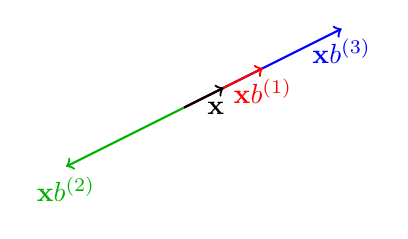
\begin{tikzpicture}
                \coordinate (O) at (0,0);
                \coordinate (X) at (0.5,0.25);
                \coordinate (A) at (1.0,0.50);
                \coordinate (B) at (-1.5,-0.75);
                \coordinate (C) at (2.0,1.00);
                \draw [->,thick,black!30!green] (O) -- (B) node[below] {$\mathbf{x}b^{(2)}$};
                \draw [->,thick,blue] (O) -- (C) node[below] {$\mathbf{x}b^{(3)}$};
                \draw [->,thick,red] (O) -- (A) node[below] {$\mathbf{x}b^{(1)}$};
                \draw [->,thick] (O) -- (X) node[pos=0.8,below] {$\mathbf{x}$};
            \end{tikzpicture}
        \end{center}
    \end{itemize}
\end{frame}

\section{Simple implementation}

\begin{frame}
    \frametitle{Numpy implementation}
    \begin{itemize}
        \item Please check \texttt{PCA.ipynb} for detailed instruction.
        % \item You will required to install \texttt{numpy}, \texttt{matplotlib}, and \texttt{jupyter notebook} as \texttt{python} packages.
    \end{itemize}
\end{frame}


\end{document}